\section{hnode Strukturreferenz}
\label{structhnode}\index{hnode@{hnode}}
{\tt \#include $<$hashtab.h$>$}

Zusammengeh\"{o}rigkeiten von hnode:\begin{figure}[H]
\begin{center}
\leavevmode
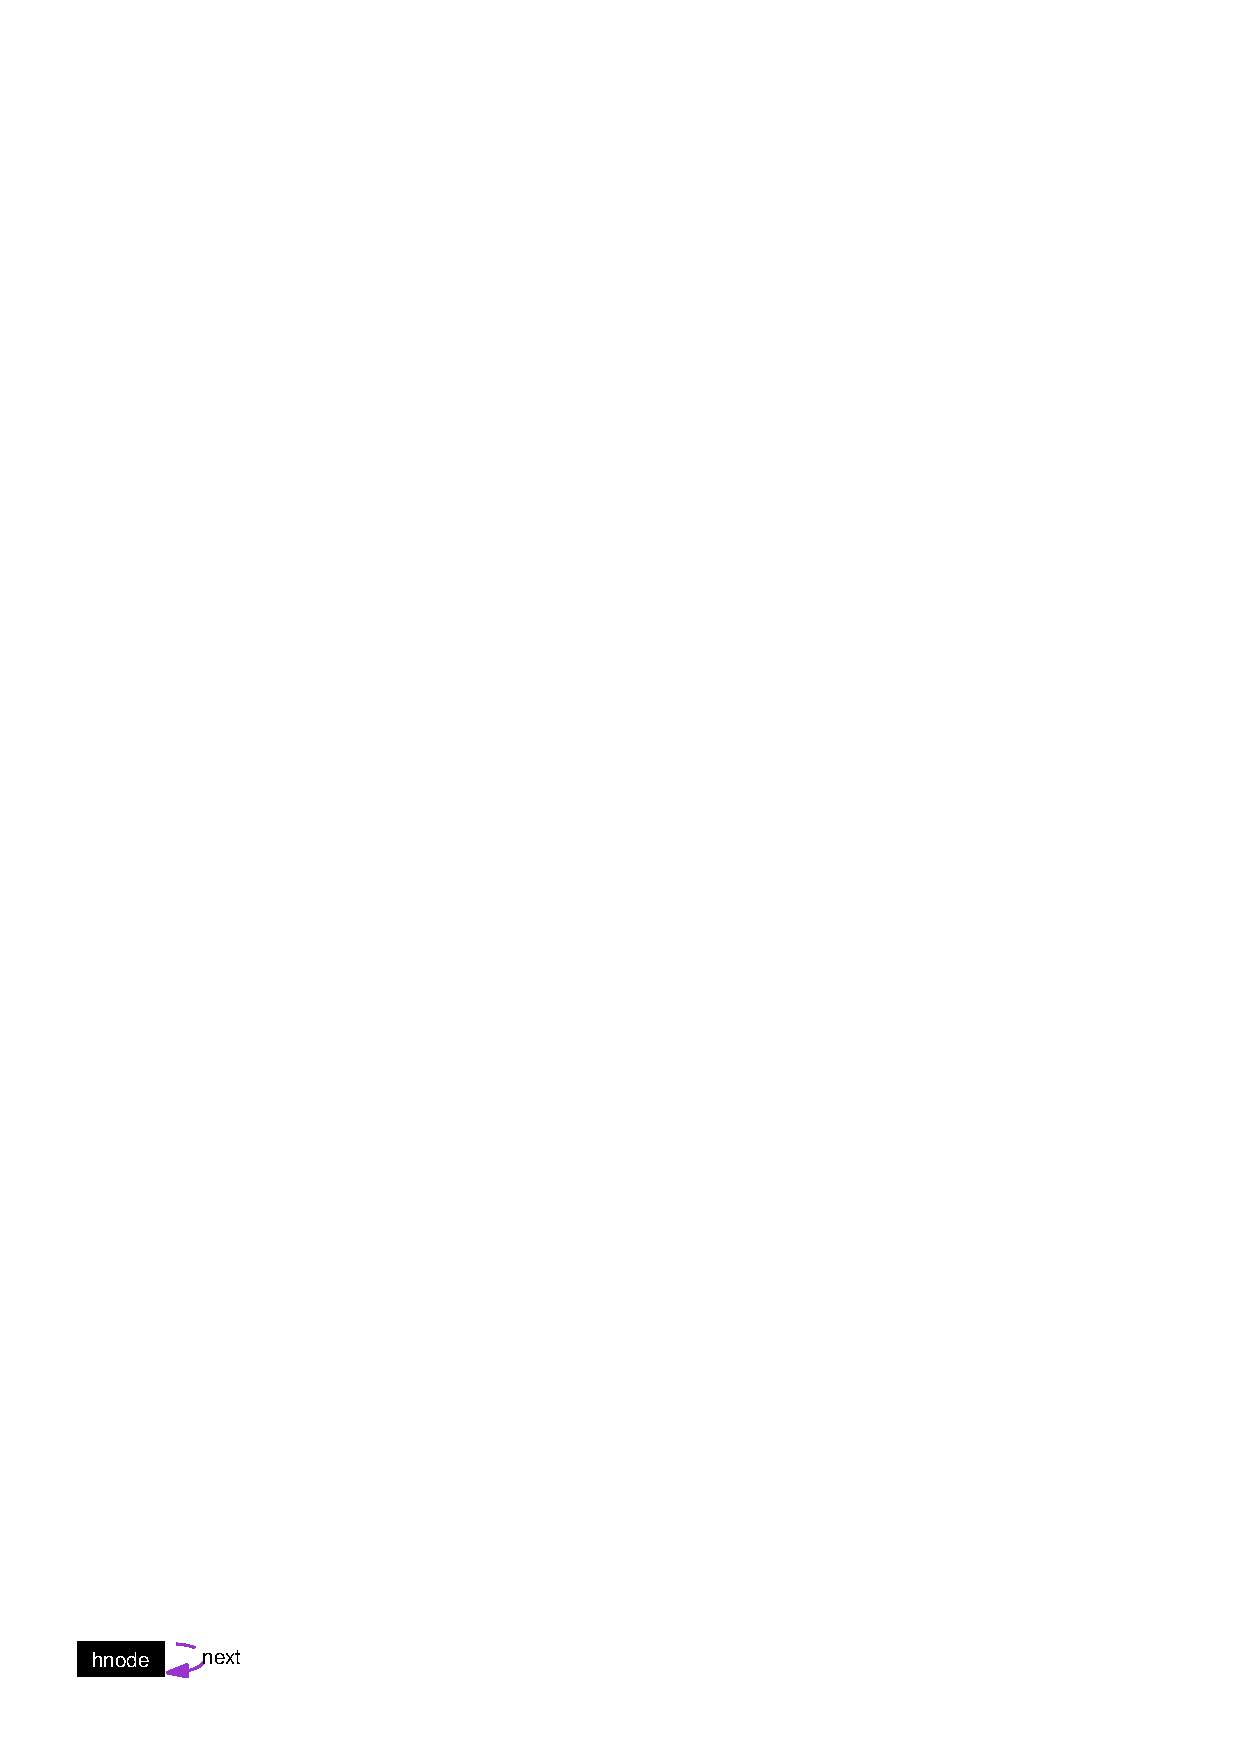
\includegraphics[width=59pt]{structhnode__coll__graph}
\end{center}
\end{figure}
\subsection*{Datenfelder}
\begin{CompactItemize}
\item 
char $\ast$ {\bf string}
\item 
int {\bf flag}
\item 
u\_\-long {\bf count}
\item 
u\_\-long {\bf files}
\item 
u\_\-long {\bf visit}
\item 
u\_\-long {\bf tstamp}
\item 
char $\ast$ {\bf lasturl}
\item 
double {\bf xfer}
\item 
{\bf hnode} $\ast$ {\bf next}
\end{CompactItemize}


\subsection{Ausf\"{u}hrliche Beschreibung}




Definiert in Zeile 26 der Datei hashtab.h.

\subsection{Dokumentation der Datenelemente}
\index{hnode@{hnode}!count@{count}}
\index{count@{count}!hnode@{hnode}}
\subsubsection{\setlength{\rightskip}{0pt plus 5cm}u\_\-long {\bf hnode::count}}\label{structhnode_ea12ded28f814b621ae07ab94aaa1f4e}




Definiert in Zeile 28 der Datei hashtab.h.

Wird benutzt von all\_\-sites\_\-page(), dump\_\-all\_\-sites(), put\_\-hnode(), top\_\-ctry\_\-table() und top\_\-sites\_\-table().\index{hnode@{hnode}!files@{files}}
\index{files@{files}!hnode@{hnode}}
\subsubsection{\setlength{\rightskip}{0pt plus 5cm}u\_\-long {\bf hnode::files}}\label{structhnode_afa2fd08fe9e22e6f183759b01a0e5c4}




Definiert in Zeile 29 der Datei hashtab.h.

Wird benutzt von all\_\-sites\_\-page(), dump\_\-all\_\-sites(), put\_\-hnode(), top\_\-ctry\_\-table() und top\_\-sites\_\-table().\index{hnode@{hnode}!flag@{flag}}
\index{flag@{flag}!hnode@{hnode}}
\subsubsection{\setlength{\rightskip}{0pt plus 5cm}int {\bf hnode::flag}}\label{structhnode_821441b6ed6dd23ac11a37d932461b03}




Definiert in Zeile 27 der Datei hashtab.h.

Wird benutzt von all\_\-sites\_\-page(), dump\_\-all\_\-sites(), month\_\-update\_\-exit(), put\_\-hnode(), top\_\-ctry\_\-table(), top\_\-sites\_\-table() und tot\_\-visit().\index{hnode@{hnode}!lasturl@{lasturl}}
\index{lasturl@{lasturl}!hnode@{hnode}}
\subsubsection{\setlength{\rightskip}{0pt plus 5cm}char$\ast$ {\bf hnode::lasturl}}\label{structhnode_d025a4c0d49fa093181202d2a91eb524}




Definiert in Zeile 32 der Datei hashtab.h.

Wird benutzt von month\_\-update\_\-exit(), new\_\-hnode() und put\_\-hnode().\index{hnode@{hnode}!next@{next}}
\index{next@{next}!hnode@{hnode}}
\subsubsection{\setlength{\rightskip}{0pt plus 5cm}struct {\bf hnode}$\ast$ {\bf hnode::next}}\label{structhnode_da1ebcc2a224afb85778f07ff89c9e23}




Definiert in Zeile 34 der Datei hashtab.h.

Wird benutzt von del\_\-hlist(), load\_\-site\_\-array(), put\_\-hnode() und tot\_\-visit().\index{hnode@{hnode}!string@{string}}
\index{string@{string}!hnode@{hnode}}
\subsubsection{\setlength{\rightskip}{0pt plus 5cm}char$\ast$ {\bf hnode::string}}\label{structhnode_eb54894424f88ea691ce2739a7b7ce80}




Definiert in Zeile 26 der Datei hashtab.h.

Wird benutzt von all\_\-sites\_\-page(), del\_\-hlist(), dump\_\-all\_\-sites(), new\_\-hnode(), put\_\-hnode(), top\_\-ctry\_\-table() und top\_\-sites\_\-table().\index{hnode@{hnode}!tstamp@{tstamp}}
\index{tstamp@{tstamp}!hnode@{hnode}}
\subsubsection{\setlength{\rightskip}{0pt plus 5cm}u\_\-long {\bf hnode::tstamp}}\label{structhnode_e02fb87d76b57ad488493862bdd54f1e}




Definiert in Zeile 31 der Datei hashtab.h.

Wird benutzt von month\_\-update\_\-exit(), new\_\-hnode() und put\_\-hnode().\index{hnode@{hnode}!visit@{visit}}
\index{visit@{visit}!hnode@{hnode}}
\subsubsection{\setlength{\rightskip}{0pt plus 5cm}u\_\-long {\bf hnode::visit}}\label{structhnode_e55f7c9efab364555b1fee0a61deb229}




Definiert in Zeile 30 der Datei hashtab.h.

Wird benutzt von all\_\-sites\_\-page(), dump\_\-all\_\-sites(), new\_\-hnode(), put\_\-hnode(), top\_\-sites\_\-table() und tot\_\-visit().\index{hnode@{hnode}!xfer@{xfer}}
\index{xfer@{xfer}!hnode@{hnode}}
\subsubsection{\setlength{\rightskip}{0pt plus 5cm}double {\bf hnode::xfer}}\label{structhnode_8069d0fba422f3b79fdeef1e263f7141}




Definiert in Zeile 33 der Datei hashtab.h.

Wird benutzt von all\_\-sites\_\-page(), dump\_\-all\_\-sites(), put\_\-hnode(), top\_\-ctry\_\-table() und top\_\-sites\_\-table().

Die Dokumentation f\"{u}r diese Struktur wurde erzeugt aufgrund der Datei:\begin{CompactItemize}
\item 
oosalizer/{\bf hashtab.h}\end{CompactItemize}
